\section{Exchange Transactions}
\label{section:exchange_transactions}

% \subsection{Markets}

% One effort to explain the sustained failure or markets to equilibriate at the aggregate level is to
% try to explain failure of equilibriation as a result of the way individual economic behaviour
% aggregates to failure or otherwise of markets for single products to equilibriate, and further to
% explain failure of markets to equilibriate at the aggregate level.
% 
% A fundamental method of science and engineering is to assume as a first step, is to use the mean
% value to aggregate a collection of micro-level behaviours. Often this turns out not to be correct,
% but invariably, in virtually every system we seek to explain, there are some parts of the system we
% explain away by averaging out noisy behaviour. 
% 
% If we use the same technique for understanding economic behaviour, we would, as a first step assume
% that we can average markets for single goods or services, result in an aggregate supply or demand
% close to zero.
% 
% If we use the same technique for understanding economic behaviour, we would, as a first step assume
% that we can aggregate our model of supply and demand for single goods or services, and arrive at a
% aggregate where aggregate supply or demand is close to zero.
% 
% Since this conclusion is contrary to facts, economists have directed their efforts at modifying the
% supply and demand model in many ways in an effort to explain this contradiction between fact and
% theory.
% 
% What is clear, however, is that the explanation has to be sufficiently fundamental to explain the
% remarkably consistent fact of excess aggregate supply and the rarity of aggregate market
% equilibrium. As put forward by Lucas, economists have yet to find a convincing understanding of
% this fact, let alone to find a solution to the problem of equilibrium failure or the problem of
% a sustained positive unemployment rate. 
% 
% Since our explanation of these facts is outside is not a part of the supply and demand model, we
% assume our simplest model of market behaviour, and that markets at the aggregate level do in fact
% equilibriate, relying on the law of large averages.

\subsection{An Exchange Transaction Only Model}

We will start with a model simplified from Figure \ref{fig:economic_feedback_schema1}. that includes only
exchange transactions.

\begin{figure}[H]
\centering
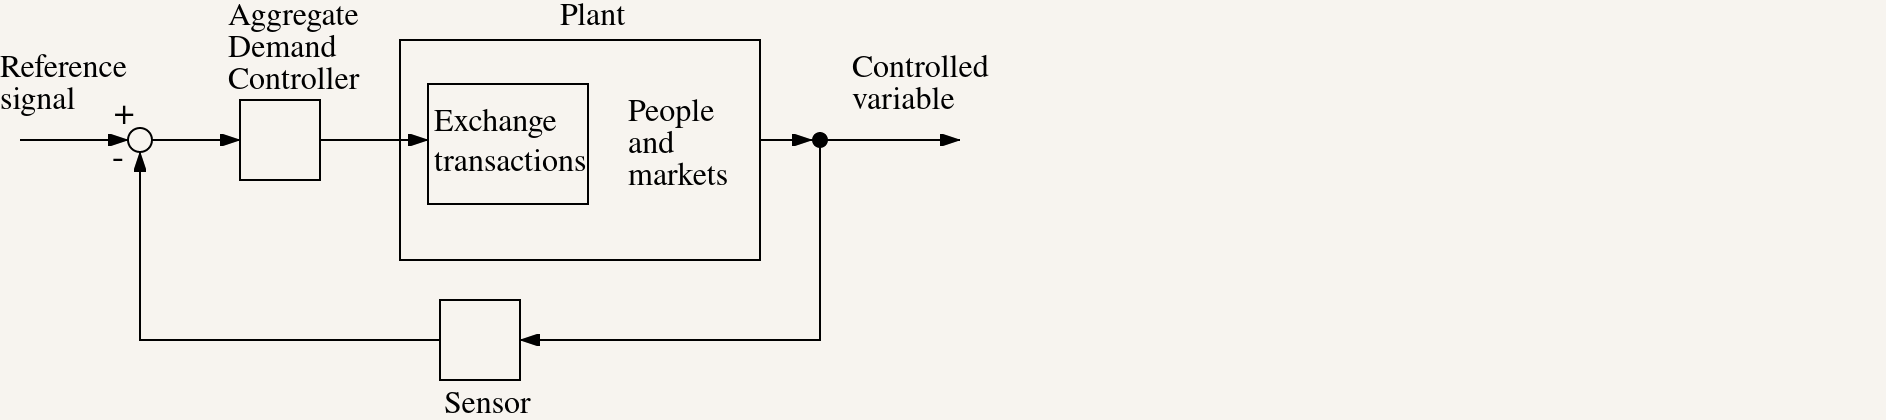
\includegraphics[scale=0.60]{03_exchange_transactions/png/exchange_only_feedback_schema}
\caption{Exchange Only Feedback Schema}
\label{fig:exchange_only_feedback_schema1}
\end{figure}

\subsection{Price and Quantity}

\begin{figure}[H]
\centering
\includegraphics[scale=0.60]{03_exchange_transactions/png/exchange_transaction}
\caption{Exchange Transaction}
\label{fig:exchange_transaction2}
\end{figure}

Exchange transactions can be quantified as a payment $p$ denominated in dollars in exchange for
quantity $q$ denominated in units specific to that good or service. We want to construct some
aggregate variables from $p$ and $q$. The term \textit{goods category} to used to refer to a
particular kind of good or service as this term more closely reflects the idea that the categories
can be redefined at various levels of specificity or generality. Using a discrete time model, for
each time period we will sum all the quantities of a given goods category $i$ so that we have a set
of $q_i$s, and collect these into a vector $\overline Q$. We'll let $N$ be the total number of
different goods categories.

\begin{equation} \label{eq:qbar}
    \overline Q = \left( q_1, \dots, q_n \right)
\end{equation}

The units for each $q_i$ are in general different. Units are denoted by enclosing in square
brackets. The units corresponding to each $q_i$ are

\[ \left( \left[ q_1 \right], \dots, \left[ q_n \right] \right) \]

The average price $p_i$ can be calculated by dividing total spending on goods category $i$ by $q_i$
and collecting them into a vector $\overline P$.

\begin{equation} \label{eq:pbar}
    \overline P = \left( p_1, \dots, p_n \right)
\end{equation}

The corresponding units for $p_i$ are

\[ \left( \left[ \frac {\$} {p_1} \right], \dots, \left[ \frac {\$} {p_n} \right] \right) \]

We cannot sum either these prices or quantities because they can have different units. But each
payment $p_i q_i$ can be summed because its unit using dimensional analysis is

\[ \left[ \frac {\$} {q_i} \right] \left[ q_i \right] = \left[ \$ \right] \]

so we will let total payments $F$, denoted in dollars, be

\[ F = p_i q_i + \dots + p_n q_n \]

What do we require of an aggregate measure of the price level? As will become clear later in the
paper (\ref{sec:constant_purchasing_power}) we require a measure of the price level $P$ that can be
used to accurately index purchasing power of a given dollar value across time. To make this more
precise consider Alice who, when she receives a dollar, purchases goods randomly selected in such a
way that in the limit, after many purchases, the distribution of her purchases is in proportion to
total transactions $\overline Q$ at that time. Suppose the price level at $t=0$ is $P_0$ and the
price level at $t=1$ is $P_1$. We want a measure of price level such that if Alice spends $1$ dollar
at $t=0$ and $P_1 / P_0$ dollars at $t=1$, then her expected value, $\overline \varepsilon_1$, of her purchases as
a proportion of $\overline Q_1$ should be equal to the expected value, $\overline \varepsilon_0$, of her
purchases as a proportion of $\overline Q_0$. In other words, we want

\begin{equation} \label{eq:p_requirement}
    \frac {P_0 \overline \varepsilon_0} {\overline Q_0} = \frac {P_1 \overline \varepsilon_1} {\overline Q_1}
\end{equation}

We will now build a measure of price from equations (\ref{eq:pbar}) and (\ref{eq:qbar}) and later
check that it agrees with equation (\ref{eq:p_requirement}). The vector $\overline Q$ represents a
collection of values, but we want to construct a single value that is a aggregate of these values.
The problem is that each of these values may have different units. We can construct units that such
as ``one apple and two oranges'' but this limits to what we can measure in these units. We can
measure ``two apples and four oranges`` but we cannot measure ``two apples and two oranges''. If we
consider only a single period of time that has $\overline Q$ transactions, then we can express
this value in any unit of the form

\begin{equation}\label{equation:basket}
    \left( \left[ \gamma q_1 \right], \dots \left[ \gamma q_n \right] \right)
\end{equation}

for any number $\gamma$. So in fact there is not just one, but a set of feasible units in which to
express $\overline Q$. We refer to any one of these set of units as a ``basket of goods''. Given
that we select one of these sets of units, we can then express $\overline Q$ as some number $Q$,
where the units given by equation (\ref{equation:basket}) with a specific $\gamma$. The units of
$Q$ is this basket of goods. Now we can set the price level as the payment for this basket of goods.
This value $P$ is in units \$ per basket. And

\begin{equation} \label{eq:fpq}
   F = PQ
\end{equation}

The units used depends on the $\overline Q$ at a point in time. If the proportion of $q_i$ changes
we would have to use a different unit, and so cannot make comparisons across time. We can solve this
problem by making use of our last degree of freedom to further constraining our units. We do set by
setting the rule that the proportion of $\gamma_1$ to $\gamma_0$ is equal to the ratio of
trade-weighted averages at times $t=1$ and $t=0$. 

\begin{equation}
    \frac {\gamma_1} {\gamma_0} = \frac {\varepsilon \left( \left[ q_1 \right], \dots, \left[ q_n \right] \right)}
    {\varepsilon \left( \left[ {q_1}' \right], \dots, \left[ {q_n}' \right] \right)}
\end{equation}

where

\[ \gamma = [q_1] \frac {f_1} F + \cdots + [q_n] \frac {f_n} F \]

Now, because $\gamma$ depends only the average of the units in the baskets of goods, the distribution of
$q_i$ around this average becomes irrelevant. This means that \textit{however} $\overline Q$
changes, whatever its distribution, the relation $F=PQ$ is exact.  

This section has involved various manipulations of units, most critically the ratio of dollar
payments to a quantity of some good or service of a collection of different quantities of goods and
services. Throughout the paper we will see that questions of units are important. Section
\ref{sec:exchange_transactions_and_errors}. will show that the price unit must change over
time. In Section \ref{section:time_transactions}. we show that the price unit written into
contracts must be constant over time. To isolate these different units and construct a control
system that has sufficient degrees of freedom required for control, the use of indices is useful.

TODO

\subsection{Aggregate Demand, Aggregate Supply and Agreements}

From equation (\ref{eq:fpq})

\[ \frac {\Delta F} F = \frac {\Delta P} P + \frac {\Delta Q} Q \]

Denoting the rate of change of the price level as the inflation rate $I$ and the rate of $Q$ as the
growth rate $G$ then

\begin{equation}
    \label{equation:fig}
    \frac {\Delta F} F = I + G
\end{equation}

Aggregate demand and aggregate demand are a set of transactions

\begin{equation}
    \sum_{i=1}^n p_i q_i
\end{equation}

Aggregate supply, $AS$, is the set of transactions that people will agree to sell if aggregate
demand is available. Aggregate demand and aggregate supply are neither well-defined or knowable
quantities as they depend on what decisions people have made in their heads. We can only measure
outomes of these variables such as $F$. The unemployment rate is a good measure of excess aggregate
supply. We are interested in aggregate supply and demand only to the extent that we can control
them. We may be able to control aggregate demand by changing the money supply. Historical experience
indicates that at some times control is effective, and at other times control is less effective. The
effectiveness of this control depends on the ability to control money supply, and the relationship
between money supply and aggregate demand. We assume that an increase in money supply will cause an
increase in aggregate demand. We want to be able to control aggregate demand through a feedback
regulator. That means that this relationship needs only to be sufficiently strong that it responds
to a feedback controller. This feedback controller may be a monetary authority or an algorithm.
Later in the paper we'll examine ways to improve this control mechanism. $AD$ and $AS$ we can derive
a set of agreements, which are the common transactions in aggregate demand and supply are is the
minimum of these two values (denominated in $\$$), and it is assumed that agreements maps directly
to transactions.

\begin{figure}[H]
\centering
\includegraphics[scale=0.48]{03_exchange_transactions/png/agreements}
\caption{Agreements as a function of aggregate supply and demand}
\label{fig:agreements}
\end{figure}

Agreements occur when both sellers and buyers want to transact and so agreements are the minimum of
aggregate supply and aggregate demand as shown in Figure \ref{fig:agreements}.

\subsection{Market Symmetry}

We assume that in aggregate economic participants drive prices and quantities in markets to an
equilibrium where $AD = AS$. This assumption is in general contrary to the economic research program
which searches for causes in deviations of fact from theory, as encapsulated by Hume's problem, in
the behaviour of market participants. One of the clearest deviations of fact from the theory of
supply and demand is the question of symmetry. The supply and demand model is symmetrical in that
there is no difference between markets being driven away from or to equilibrium as a result of
excess demand or markets being drive away from or to equilibrium as a result of excess supply, 

\begin{figure}[H]
\centering
\includegraphics[scale=0.48]{03_exchange_transactions/png/symmetry}
\caption{Symmetric Market Model}
\label{fig:symmetric_market_model}
\end{figure}

The right hand side of Figure \ref{fig:symmetric_market_model} is a diagrammatic representation of
what the outcome of the symmetric market model should look like in measurements of the unemployment
rates. Any measurement that represent excess aggregate demand will be mapped to an unemployment rate
of zero or close to zero. Half the data-points should therefore sit close to an unemployment rate of
zero. This model is inconsistent with many decades of unemployment data.
